% 简谐振子受迫运动
% 简写振子|受迫运动|受迫|幅频曲线|相频曲线

\pentry{受阻简谐振子\upref{SHOf}, 振动的指数形式\upref{VbExp}}

在受阻简谐振子的基础上, 若给振子额外施加一个周期变化的力(驱动力), 得到微分方程如下.
\begin{equation}\label{SHOfF_eq1}
m\ddot y = -\alpha \dot y - ky + f(t)
\end{equation}
以下只讨论 $f(t)$ 为简谐函数的情况, 令其振幅为 $B$, 频率为 $\omega$. 我们姑且假设经过足够长的时间后, 该弹簧振子也会做简谐振动, 振动频率等于 $f(t)$ 的频率. 若能找到一个这样的解, 就说明该假设是对的.

为了方便计算, 我们用指数形式表示振动, 设
\begin{equation}
\tilde y(t) = \tilde A\E^{-\I\omega t} \qquad
\tilde f(t) = \tilde B\E^{-\I \omega t}
\end{equation}
由于我们的微分方程是线性的, 如果复数形式的 $y(t)$ 和 $f(t)$ 能满足微分方程, 那么它们的实部也能满足该微分方程. 将它们代入\autoref{SHOfF_eq1}, 得
\begin{equation}
\tilde A =  \frac{\tilde B}{k -\omega^2 m - \I\alpha\omega}
\end{equation}
由于弹簧振子的固有频率为 $\omega_0 = \sqrt{k/m}$, 上式可用 $\omega_0$ 表示为
\begin{equation}
\tilde A = \frac{\tilde B}{m(\omega_0^2 - \omega^2) - \I\alpha\omega}
\end{equation}
上式两边求模长, 得到简谐振子的振幅 $A = |\tilde A|$ 与驱动力频率 $\omega$ 的关系, 称为\textbf{幅频关系}
\begin{equation}\label{SHOfF_eq5}
A = \frac{B}{\sqrt{(\omega^2 - \omega_0^2)^2 m^2 + \alpha^2\omega^2}}
\end{equation}
假设 $\tilde B$ 的幅角为零, 对 $\tilde A$ 求负幅角, 得简谐振子初相位 $\varphi_0$ 与驱动频率 $\omega$ 的关系, 称为\textbf{相频关系}($\arctan2$ 的定义见%未完成
)
\begin{equation}\label{SHOfF_eq6}
\varphi_0 = -\arg \tilde A = \arctan2 \qty[m(\omega_0^2 - \omega^2), -\alpha\omega]
\end{equation}

%未完成:复数复习词条中, 要提如何求幅角, 如何把分母变为实数, 如何计算复数相除
\begin{figure}[ht]
\centering
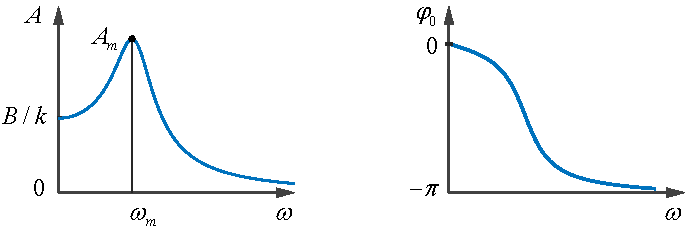
\includegraphics[width=12cm]{./figures/SHOfF1.pdf}
\caption{幅频曲线和相频曲线} \label{SHOfF_fig1}
\end{figure}

\autoref{SHOfF_eq5} 的根号内是关于 $\omega^2$ 的二次函数, 求得二次函数最小值的位置为
\begin{equation}
\omega_m = \sqrt{\omega_0^2 - \frac{\alpha^2}{2m^2}}
\end{equation}
幅频曲线可改写为
\begin{equation}\label{SHOfF_eq8}
A = \frac{B}{m\sqrt{(\omega^2 - \omega_m^2)^2 + (\omega_0^4 - \omega_m^4)}}
\end{equation}
所以 $A$ 的最大值为
\begin{equation}
A_m = \frac{B}{m\sqrt{\omega_0^4 - \omega_m^4}}
\end{equation}
由\autoref{SHOfF_eq8} 可得, 当 $\omega = 0$ 和 $\omega\to +\infty$ 时, 振幅分别为 $B/k$ 和 $0$. 前者代表施加的是一个恒力, 结论符合胡克定律.

再来观察相频曲线, 注意初相位始终为负, 说明简谐运动的相位始终落后于驱动力的相位, 且频率越快, 落后越多. 由\autoref{SHOfF_eq6} 可知当 $\omega\to +\infty$ 时相位恰好落后 $\pi$.



